\documentclass[10pt]{article}
\usepackage[margin=1in]{geometry}
\usepackage{mathptmx}
\usepackage[T1]{fontenc}
\usepackage{amsmath,amssymb,bm}
\usepackage{graphicx}
\usepackage{booktabs}
\usepackage{xcolor}
\usepackage{microtype}
\usepackage{enumitem}
\usepackage[numbers,sort&compress]{natbib}
\usepackage[font=small,labelfont=bf,labelsep=colon,skip=3pt]{caption}
\usepackage[colorlinks=true,linkcolor=blue!50!black,citecolor=blue!50!black,urlcolor=blue!50!black]{hyperref}
\setlist{itemsep=1pt,topsep=2pt,parsep=0pt,leftmargin=1.5em}
\setlength{\parskip}{2.5pt}
\setlength{\parindent}{0pt}
\renewcommand{\bibfont}{\small}
\setlength{\bibsep}{1pt}
\renewcommand{\topfraction}{0.95}
\renewcommand{\bottomfraction}{0.9}
\renewcommand{\textfraction}{0.08}
\renewcommand{\floatpagefraction}{0.75}
\newcommand{\Hess}{\mathbf{H}}
\newcommand{\jl}{J_\ell}
\newcommand{\figref}[1]{Figure~\ref{#1}}
\newcommand{\secref}[1]{\S\ref{#1}}
\title{\vspace{-1.2em}Can Curvature Help Interpret Language Models?\\Extending the Jacobian Lens to Second Order}
\author{Manuel Villanueva\\\texttt{manuel@villanuev.com}}
\date{}

\begin{document}
\maketitle
\vspace{-2.2em}
\begin{abstract}
\small
The Jacobian lens (J-lens) reads what a language model is poised to say from an activation, using one first-order map per layer; the interventions built on it (concept swaps, steering, ablation) are linear in the activation. Many phenomena it is used to study are nonlinear, which raises a concrete question: what does second-order structure add? We build an ``H-lens'' toolkit around Hessian-vector products through layer slices, restricted Hessians over J-lens directions, a trust score for the perturbations actually applied, and a reliability harness (estimator agreement, Taylor-validity checks, weight-randomized controls). We use it to test ten of twelve hypotheses on Qwen3.5-4B, Gemma~3~12B and Llama~3.1~8B (Qwen3.6-27B, in mixed precision validated for one measurement, for one claim). The hypotheses were fixed in internal, hash-recorded pre-registrations; several tests were designed after earlier data, and the Gemma swap strength was chosen post hoc.
We find one robust positive result: the curvature of the MLP branch along J-lens directions exceeds its curvature along random directions in the upper layers of all three models (median ratios up to 2.2, 13.0 and 2.8 at the last measured layer), whereas weight-randomized models show none (15 control arms within 0.6\% of 1). Variance-matched control directions do not remove the effect, but unembedding directions (the lens vectors without the Jacobian) carry nearly all of it (lens/unembedding ratio 1.05 on Gemma, 1.16 and 1.32 on Qwen and Llama), so the effect is a property of token-aligned directions more than of the Jacobian map.
For interventions, the \emph{local linearization} of the answer margin along a concept swap ranks which swaps succeed better than the nonlinear remainder does (AUC 0.65 on Qwen, 0.81 on Gemma, against 0.51 and 0.25), but it also flags many swaps that do not succeed (precision 0.47--0.56), swap success is threshold-like, and the second-order trust score tracks the size of the first-order push rather than flagging failures.
A second-order mutual-inhibition effect at the ignition threshold holds on Qwen3.5-4B only; it fails on Gemma~3~12B and Qwen3.6-27B. Binding, remainder coupling, early-layer content, motor-regime collapse, load-dependent competition and a persona-specific signature are not supported, and one first-pass dissociation (persona versus register) did not survive scaling. A context-free MLP-gain check of the original work did not reproduce on Qwen3.5-4B.
\end{abstract}

\section{Introduction}
Interpretability tools built on gradients treat a network as locally linear. The Jacobian lens (J-lens) is a clean example~\citep{gurnee2026workspace}: for each layer $\ell$ it averages the input--output Jacobian of the final residual stream over a corpus of contexts and positions, and reads an activation $h_\ell$ as $\mathrm{lens}(h_\ell)=\mathrm{softmax}(W_U\,\mathrm{norm}(\jl h_\ell))$. The rows of $W_U\jl$ are the \emph{J-lens vectors}, one per vocabulary token. Reading is linear in $h_\ell$, and so is every operation the lens supports: steering along a lens vector, ablating it, or swapping two concepts in lens coordinates, $h\leftarrow h+V(\sigma(c)-c)$ with $c=V^{+}h$.

\begin{figure}[!t]
\centering
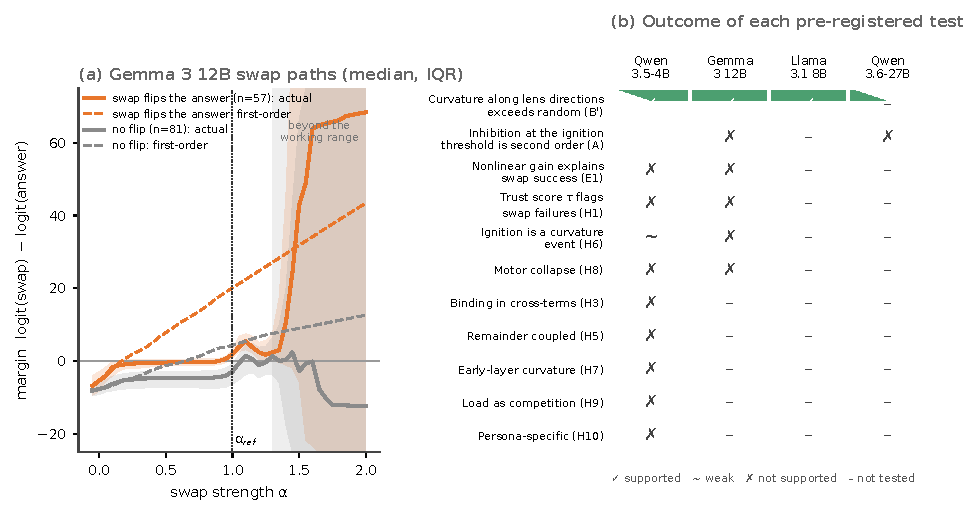
\includegraphics[width=6.50in]{figures/fig_overview.pdf}
\caption{\textbf{Summary.} (a) Answer-margin paths along a concept swap on Gemma~3~12B (median and interquartile range over the 57 items whose answer flips at $\alpha=1.0$ in the margin-path run and the 81 that do not; the swap suite of Figure~\ref{fig:swap} counts 55). The first-order extrapolation (dashed) ranks the items; the actual margin is flat, crosses zero near $\alpha\approx1$, and rises sharply only beyond the swap strengths at which the intervention is meant to work (``working range'', $\alpha>1.3$ here, shaded). (b) Outcome of each hypothesis test by model (hypothesis names as in Table~\ref{tab:hyp}): supported (\checkmark), weak ($\sim$), not supported ($\times$), not tested ($-$).}
\label{fig:overview}
\end{figure}

\subsection{Motivation: a first-order tool for nonlinear questions}
The linear construction is the lens's strength (it is cheap, context-independent and grounded in the model's own derivatives) and also its blind spot. The questions the original work leaves open are largely nonlinear: what the sharp ``ignition'' of a concept is mechanistically, why the workspace holds only tens of concepts, whether the broad broadcast of lens directions through the weights reflects alignment or nonlinear amplification, whether early layers are empty or merely linearly inaccessible, and how concepts are bound rather than merely present. In the attribution literature the same tension is documented: AtP* catalogues the failure modes of first-order attribution patching~\citep{kramar2024atp}, and a recent analysis attributes its dominant error to nonlinearities downstream of the patched site and corrects it with one Hessian-vector product~\citep{zhang2026lies}. If intervention results on the J-lens inherit that limit, some of what looks like workspace structure could be linearization error, and some real structure could be invisible to the lens.

\subsection{The H-lens: adding the next Taylor term}
We ask whether second-order structure adds explanatory power to the J-lens, and build the machinery to answer it. For a map $f$ (a slice of layers, or a layer-to-logit map) we never materialize the Hessian; we fix a contraction and compute Hessian-vector products (HVPs)~\citep{pearlmutter1994fast}. We use three quantities: (i) the \emph{restricted Hessian} $H_{ij}=v_i^\top \Hess v_j$ over a few J-lens directions, whose off-diagonal terms measure interaction between concepts; (ii) the \emph{trust score} $\tau=\|\tfrac12\delta^\top\Hess\delta\|/\|J\delta\|$ for the perturbation $\delta$ actually applied, the ratio of the second- to the first-order change; and (iii) the curvature $\kappa(v)=\|\tfrac12 v^\top\Hess v\|$ of the MLP branch along a unit direction. None of these is reported without a validity gate and a weight-randomized control (\secref{sec:methods}).

\subsection{What we find}
We registered twelve hypotheses (H1--H11 and a follow-up, E1; Table~\ref{tab:hyp}); ten could be run, and two need training checkpoints we do not have. We ran them on three architectures: a hybrid linear/full-attention model (Qwen3.5-4B), a model with sliding and global attention (Gemma~3~12B), and a dense decoder (Llama~3.1~8B); Qwen3.6-27B was used for one claim. \figref{fig:overview} summarizes the outcomes. In brief:
\begin{itemize}
\item \textbf{Curvature along lens directions is real (\secref{sec:bprime}).} In the upper layers, $\kappa$ along J-lens directions exceeds $\kappa$ along random directions on all three models, and weight-randomized controls show no effect. Variance-matched controls leave the effect intact, but unembedding directions without the Jacobian carry most of it.
\item \textbf{Local linearization ranks swap outcomes, but swaps are not linear (\secref{sec:suffice}).} Concept swaps are causal and control-separated on both models tested, with a model-dependent best strength and threshold-like success. Which swaps succeed is ranked by the first-order extrapolation of the answer margin better than by the nonlinear remainder, though the extrapolation also flags many swaps that fail, and $\tau$ marks the size of the first-order push, not failure.
\item \textbf{One second-order effect is specific to one 4B model (\secref{sec:claima}).} Near the ignition threshold (where an interpolated concept embedding makes the model switch its answer), raising one concept lowers the sensitivity of a competing one (negative second-order cross-terms against positive first-order cross-effects) on Qwen3.5-4B only.
\item \textbf{Most second-order hypotheses fail (\secref{sec:negatives}).} Binding, remainder coupling, early-layer content, motor-regime collapse, load-dependent competition and a persona-specific signature are not supported; the ignition-as-curvature hypothesis is weak on Qwen and absent on Gemma.
\end{itemize}

\subsection{Takeaways}
Second-order structure is present and aligned with the lens's directions, but for the interventions we could test it is not where the explanatory power is: the local first-order extrapolation ranked swap outcomes and the nonlinear remainder did not. We do not claim that swaps are linear; success is threshold-like and the first-order prediction has many false alarms. For lens users, swap outcomes are better predicted by first-order quantities of the intervention itself than by second-order ones. For the second-order program, most hypotheses that attribute a mechanism to curvature fail under controls, and the exceptions (curvature along lens directions; one inhibition effect on one model) describe structure rather than demonstrate use.

\section{Methods}
\label{sec:methods}
\subsection{The Jacobian lens and concept swaps}
We use the corpus-averaged Jacobian $\jl=\mathbb{E}_{t,t'\ge t,\mathrm{prompt}}[\partial h_{\mathrm{final},t'}/\partial h_{\ell,t}]$ and its readout as defined in \citet{gurnee2026workspace}, with the pre-fitted lenses distributed through Neuronpedia~\citep{neuronpedia2026lenses}. It generalizes the logit lens ($\jl=I$)~\citep{nostalgebraist2020logit} by correcting for representational change across layers, and differs from the tuned lens~\citep{belrose2023tuned} in being a causal average rather than a trained predictor. A \emph{swap} exchanges two concepts in lens coordinates: with $V=[v_s\;v_t]$ the raw lens vectors, $c=V^{+}h$ and $\sigma$ the exchange, $h\leftarrow h+\alpha V(\sigma(c)-c)$, applied at every position over a band of layers with one editor per layer, since each layer has its own $\jl$. Success means the greedy next token equals the swapped answer. The J-space component of an activation is found by sparse non-negative decomposition over the lens vectors (non-negative matching pursuit, a gradient-pursuit variant~\citep{mallat1993matching,blumensath2008gradient}); we use it in the sparse-atom tests (H5) and a reproduction check. We use the lenses as distributed (Table~\ref{tab:models}); the only lenses we fit are the null lenses and one control in \secref{sec:bprime}.

\subsection{Second-order objects}
Let $f$ map the layer-$\ell$ residual to a scalar or vector. We compute HVPs with three estimators: reverse-over-reverse (reference), forward-over-reverse (production, no double graph~\citep{baydin2018automatic}) and central finite differences (validation only). The restricted Hessian over directions $\{v_i\}$ costs $k$ HVPs. For the trust score the Hessian enters as one Jacobian-vector product of a Jacobian-vector product, with no contraction choice; the perturbation $\delta$ is the swap delta itself, since a score evaluated on perturbations nobody applies says nothing about the interventions' reliability. We read $\tau$ at several layers $\ell$, with $f$ the final-layer residual at the answer position.
Three measurements recur. \emph{Curvature ratio:} $\kappa$ of the MLP branch (its own norms included) at layer $\ell{+}1$ for unit directions drawn from three populations: lens vectors of tokens actually active on text, MLP-neuron output directions, and isotropic random directions; the ratio is the median over lens directions divided by the median over random directions, per layer. \emph{Ignition protocol:} the embedding at a slot is interpolated, $(1-\alpha)e_B+\alpha e_A$, between two country words; the model's answer switches sharply at a threshold $\alpha^*$ (``ignition''), defined as where the projection share of the activation on concept $A$ at a mid layer crosses $0.5$. \emph{Inhibition:} at $\alpha^*$ and $\alpha^*\pm0.2$ we form the restricted Hessian of two readouts (unit lens vectors of the two countries at a target layer) over the two concepts' lens directions at a source layer; with cross-terms $c_A,c_B$, inhibition is $I=-(c_A+c_B)/2$.

\begin{figure}[!t]
\centering
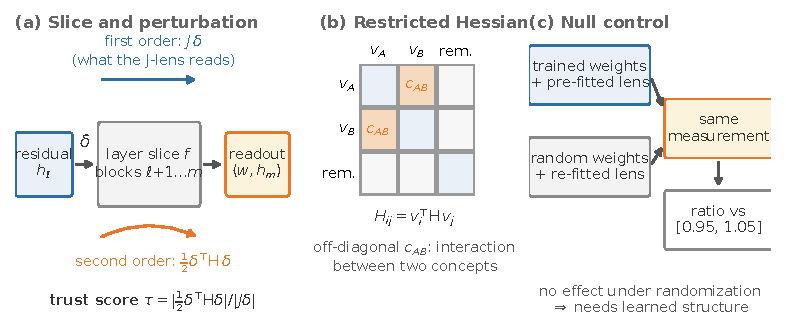
\includegraphics[width=5.24in]{figures/fig_schematic.pdf}
\caption{\textbf{The H-lens objects.} (a) For a perturbation $\delta$ of the layer-$\ell$ residual, the J-lens sees the first-order change $J\delta$ of a downstream readout; the H-lens adds the second-order term $\tfrac12\delta^\top \mathrm{H}\delta$ of the layer slice, and the trust score $\tau$ is their ratio, evaluated on the perturbations interventions actually apply. (b) The restricted Hessian over a few lens directions (here two concepts and the non-J-space remainder): off-diagonal entries measure interaction. (c) Every curvature measurement is repeated on a weight-randomized copy with a lens re-fitted on it.}
\label{fig:schematic}
\end{figure}

\subsection{Reliability harness and controls}
Every curvature number passes four gates. (i) \emph{Estimator agreement:} the three HVP estimators agree on analytic quadratics, a small MLP against exact Hessians, and on real slices in fp32 (relative difference $1.2\times10^{-6}$ on Llama, $5.5\times10^{-7}$ on Gemma, $\sim10^{-6}$ on Qwen). (ii) \emph{Exact slices:} the pure layer-slice function reproduces the hooked forward pass to zero difference on every model; this required per-block capture of rotary embeddings and masks, because hybrid and sliding-window architectures differ by block. (iii) \emph{Taylor validity:} a finite-difference plateau gives a Taylor radius, and a validity score below one flags that the quadratic picture has broken down at the step size used; Lanczos eigenvalue estimates are checked against longer runs. (iv) \emph{Weight-randomized null:} we re-initialize the model with the library's own initialization, round to bf16 precision, \emph{re-fit a lens on the randomized weights}, and run the identical pipeline. The pre-fitted lens is meaningless on random weights, so a faithful null repeats the whole procedure~\citep{adebayo2018sanity}. For claims of no effect we use an equivalence test~\citep{lakens2017equivalence}: the whole 95\% interval of the null ratio must lie in $[0.95,1.05]$.

\subsection{Models, precision and depth matching}
\begin{table}[!t]
\centering\small
\begin{tabular}{@{}p{3.0cm}p{1.9cm}p{3.3cm}p{1.6cm}p{2.6cm}@{}}
\toprule
Model (checkpoint) & Layers / $d$ & Attention & Lens prompts & Used for \\
\midrule
Qwen3.5-4B~\citep{qwen2026models} & 32 / 2560 & 3:1 Gated DeltaNet~\citep{yang2025gated} : full & 417 & all tests \\
Gemma 3 12B (\texttt{-pt})~\citep{gemmateam2025gemma3} & 48 / 3840 & sliding : global & 775 & most tests \\
Llama 3.1 8B (base)~\citep{llamateam2024llama3} & 32 / 4096 & dense, GQA & 539 & curvature ratio \\
Qwen3.6-27B~\citep{qwen2026models} & 64 / 5120 & 3:1 hybrid & 1000 & inhibition (mixed prec.) \\
\bottomrule
\end{tabular}
\caption{Models. All four are the base or pre-trained checkpoints (\texttt{Qwen/Qwen3.5-4B}, \texttt{google/gemma-3-12b-pt}, \texttt{meta-llama/Llama-3.1-8B}, \texttt{Qwen/Qwen3.6-27B}). The lenses are the pre-fitted files of \texttt{neuronpedia/jacobian-lens}~\citep{neuronpedia2026lenses}, fitted on WikiText-103 prompts (bf16, 128 tokens) with a convergence-based stop of at most 1000 prompts; ``Lens prompts'' is the number each fit used. We did not refit them. All curvature work is fp32 with eager attention, since fused kernels lack forward-mode autodiff.}
\label{tab:models}
\end{table}
All curvature results use fp32 weights; bf16 rounding swamps second differences. The 27B model does not fit in fp32 ($\approx108$\,GB), so it is held in bf16 with fp32 copies of only the HVP slice, the final norm and the output head~\citep{micikevicius2018mixed}; this path reproduced the fp32 inhibition result on Qwen3.5-4B (sign agreement 98.6\%/100\%, Spearman 0.999 over 72 cells, median relative error 0.34\%) but was validated for that measurement only. Absolute layer numbers do not transfer between architectures, so every layer is mapped by depth fraction, $\ell/(L{-}1)$, to its counterpart on the reference model; we report depth explicitly. Text contexts are WikiText prompts~\citep{merity2017pointer}.

\subsection{Pre-registration and statistics}
Each hypothesis has a file fixing setup, tests and decision rule before data; result files store its SHA-256, and a real arm refuses to run before the randomized arm under the same hash~\citep{nosek2018preregistration}. Deviations are dated addenda. The registrations are internal (same team, hash-recorded files, not an external registry). Tests: AUC with bootstrap intervals~\citep{efron1979bootstrap}; one- and two-sided permutation, Wilcoxon signed-rank~\citep{wilcoxon1945individual} and Mann--Whitney~\citep{mann1947test} tests; Spearman correlation~\citep{spearman1904proof}; Wilson intervals~\citep{wilson1927probable}; stratified tests (geography relations versus others, defined after the first analysis); prompt- and pair-level cluster bootstraps; Bonferroni correction for multi-configuration scans. The unit of each analysis is stated with its result: prompts (the B$'$ intervals, 30 prompts with 16 contexts each), items (swap and trust-score tests; items sharing a relation or entities are not independent, so we add stratified tests), trials (inhibition and ignition tests; a trial is one carrier template with one country pair, and templates and words are reused, so these $p$-values are optimistic) and pairs (H10; two carriers averaged).

\section{Results}
Table~\ref{tab:hyp} lists the hypotheses and the quantity that tests each. We first reproduced the original work's first-order checks on the open models (Appendix~\ref{app:gates}); the main departures are that the context-free MLP-gain gate was not reproduced on Qwen3.5-4B and that the swap rate depends strongly on strength $\alpha$ and model.

\begin{table}[!t]
\centering\footnotesize
\begin{tabular}{@{}p{0.9cm}p{5.6cm}p{4.3cm}p{3.7cm}@{}}
\toprule
 & Hypothesis & Test quantity & Outcome \\
\midrule
B$'$ (H2) & Curvature along lens directions exceeds random & $\kappa$ ratio; equivalence-tested null & holds on 3 models \\
A (H9, part 1) & Competing concepts inhibit each other at the ignition threshold & inhibition $I$; cross-terms & Qwen3.5-4B only \\
H1 & The trust score $\tau$ flags swap failure & AUC of $\tau$ & no ($\tau$ marks success) \\
E1 & Nonlinear gain explains swap success & AUC of $N$ versus $FO$ & no; $FO$ ranks success \\
H6 & Ignition is a curvature event & Lanczos $\lambda$ along the path & weak (Qwen), no (Gemma) \\
H8 & Curvature collapses near the output & per-block nonlinearity & no \\
H3, H5 & Binding in cross-terms; remainder coupled to atoms & $|H_{ij}|$ rank; remainder cross-terms & no \\
H7, H9-load & Curvature carries early-layer content; competition grows with load (H9, part 2) & probe; inhibition vs load & no \\
H10 & Persona-specific ignition signature & pair-level effect, matched control & no \\
H4, H11 & Automatization; reflection training & needs checkpoints & not run \\
\bottomrule
\end{tabular}
\caption{Hypotheses, the quantity that tests each, and the outcome (details in the sections that follow).}
\label{tab:hyp}
\end{table}

\subsection{Curvature along lens directions exceeds random directions}
\label{sec:bprime}
Our first formulation (B) asked whether $\kappa$ along lens directions is above random with a null interval containing 1; it failed its own rules, because bootstrap intervals about $\pm0.0005$ wide around ratios of 0.997--1.002 exclude exactly 1 (Appendix~\ref{app:b}). We replaced the null rule by the equivalence margin $\delta=0.05$ and re-pre-registered on fresh prompts and seeds (B$'$).

\begin{figure}[!t]
\centering
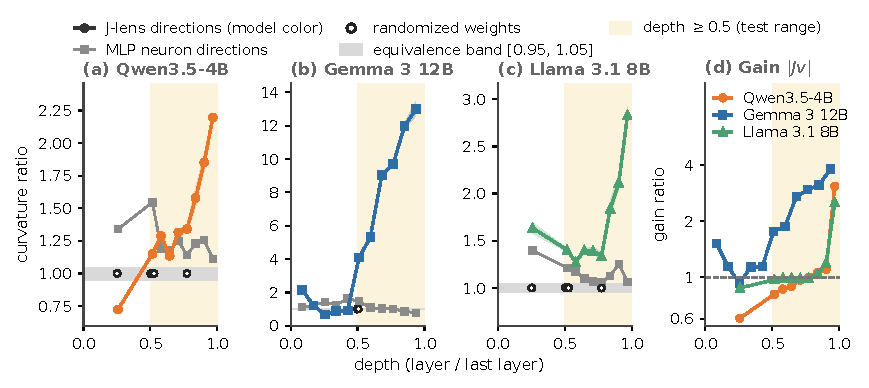
\includegraphics[width=5.79in]{figures/fig_bprime.pdf}
\caption{\textbf{Curvature along J-lens directions exceeds random directions in the upper layers, and weight-randomized models show none.} (a--c) Median ratio of $\kappa$ along lens directions to $\kappa$ along random directions, per layer (orange/blue/green with 95\% prompt-cluster intervals), against MLP-neuron output directions (gray) and against the same pipeline on weight-randomized models with a re-fitted lens (open circles, one per seed and layer; shaded gray: equivalence band $[0.95,1.05]$). The shaded yellow region is the depth range $\ge0.5$ used for the test. (d) The first-order gain ratio $\|Jv\|$ for the three models (dashed line: ratio 1; log scale): on Qwen and Llama curvature is raised while first-order gain is not (until the final layers); on Gemma both are raised.}
\label{fig:bprime}
\end{figure}

B$'$ holds on all three models (\figref{fig:bprime}). Every null arm lies inside $[0.95,1.05]$ (15 arms: 5, 5 and 5 on Qwen3.5-4B, Gemma~3~12B and Llama~3.1~8B; ratios 0.9994--1.0052, three Gemma seeds having been added after review; the 8 arms of the first formulation in Appendix~\ref{app:b} give 0.994--1.002, 23 arms in all), the real lower bound exceeds 1.05 at every measured layer at depth $\ge0.5$ (8/8, 6/6 and 8/8), and at the matched null layers it exceeds every null arm's upper bound. The median ratios over that range are 1.33 on Qwen (rising from 1.15 at L16 to 2.20 at L30), 9.4 on Gemma (4.1 at L24 to 13.0 at L44) and 1.40 on Llama (1.40 at L16 to 2.83 at L30), so only Gemma qualifies as ``large'' by the 1.5 label we inherited from formulation B. A median over layers hides the trend: on Qwen and Llama the ratio exceeds 1.5 only in the last few layers, and on Gemma from depth 0.5 on. MLP-neuron output directions are mildly elevated on Qwen and Llama (1.06--1.55) and the lens ratio exceeds them at 6 of 8 layers on Qwen, all 8 on Llama and all 6 on Gemma. The first-order gain ratio (\figref{fig:bprime}d) is near 1 up to the last layers on Qwen and Llama but rises early on Gemma, so curvature and gain dissociate on two models and not on the third. Normalizing by the gain, the median ratio of $\rho=\kappa\|r\|/\|Jv\|$ (second- to first-order change for a perturbation as large as the activation) along lens directions over random ones is 1.29 on Qwen, 3.18 on Gemma and 1.32 on Llama, so part of Gemma's larger effect reflects its larger first-order gain along lens directions, but a threefold gain-normalized curvature enrichment remains.
\textbf{Controls added after B$'$.} An isotropic baseline leaves four alternatives open, so we added control populations in a further registration, designed after seeing B$'$ (Appendix~\ref{app:controls}, Table~\ref{tab:controls}). \emph{Variance:} for each lens direction we picked the activation-covariance or isotropic direction whose variance of the residual along it is closest. Lens-to-matched ratios are 1.32 (Qwen), 9.2 (Gemma) and 1.40 (Llama), with lower bounds above 1.05 at every layer, so alignment with high-variance directions does not explain the effect. \emph{Token directions:} unembedding directions without the Jacobian have almost the same curvature on Gemma (lens/unembedding 1.05; the pre-registered test fails there) and only slightly less on Qwen and Llama (1.16 and 1.32, test passes), and input-embedding rows lie in between (6.7, 1.17 and 1.40). Most of the enrichment is therefore a property of token-aligned directions, and the Jacobian map adds a factor of at most about 1.3. \emph{Activation covariance} (descriptive): directions sampled from the second-moment matrix of the residual have about the curvature of lens directions on Qwen below layer 28 (ratio 1.01), much less on Gemma (129$\times$ lower) and somewhat less on Llama (1.26). \emph{Lens fit:} refitting the real lens with the 30-prompt null recipe gives ratios of 1.16 and 1.38 at L16 and L24 on Qwen (1.15 and 1.34 with the distributed lens) and 4.18 at L24 on Gemma (4.09), so the lens-fit recipe does not explain the contrast with the null arms.
\textbf{What this says:} curvature of the MLP branch is raised along token-aligned directions, which include lens directions, in trained networks and not in randomized ones. \textbf{What it does not say:} that the lens's Jacobian is what makes the directions special, or that the model uses the curvature. We designed B$'$ after seeing B's data; the pre-registered margin, fresh prompts and new seeds are what make it a test.

\subsection{Local linearization ranks swap outcomes, but swaps are not linear}
\label{sec:suffice}
\textbf{Swaps are causal on both models, at model-dependent strengths.} On the original 87-item suite, the swap flipped 35\% of baseline-correct items on Qwen3.5-4B (the original work reports 54--70\% on Claude models) against 0/52 for random-direction swaps; we had tuned the band and $\alpha$ on those items. We therefore generated a held-out suite of 165 two-hop items from fact tables (city $\to$ country $\to$ capital, language, continent or currency; element $\to$ symbol or state; language $\to$ country $\to$ capital) with single-token entities in both tokenizers, disjoint from the original, and fixed the protocol in advance. Qwen's rate held up (61/125 = 48.8\% at the tuned $\alpha=1.25$, controls 0/0/0). On Gemma~3~12B the pre-registered $\alpha=1.25$ failed (5/138 = 3.6\%). The strength $\alpha=1.0$, which we had chosen post hoc on the first suite, reached 55/138 = 39.9\% on the held-out items (Figure~\ref{fig:swap}, Appendix~\ref{app:swap}); this confirms the strength out of sample but is not a pre-registered pass. The steep drop between $\alpha=1.0$ and $1.25$ is already a sign of threshold behavior.


\textbf{What predicts success.} The E1 and H1 analyses re-run the swap path item by item; they count 57 flips of 138 baseline-correct items on Gemma at $\alpha=1.0$ and 61 of 126 on Qwen at $\alpha=1.25$, where the swap suite above counts 55 of 138 and 61 of 125. The two runs differ by a few items, which we did not trace. For each baseline-correct item we measure the answer margin $m(\alpha)=\mathrm{logit}(\text{swap})-\mathrm{logit}(\text{answer})$ along the swap path ($\alpha$ from $-0.05$ to $2.0$). Three derived quantities matter. The first-order extrapolation $FO(\alpha)=m(0)+\alpha\,m'(0)$ is the local linearization of this one margin, with $m'(0)$ from a central difference; it is the true local derivative along this swap, not the corpus-averaged lens. The nonlinear remainder $N=m(\alpha_{\mathrm{ref}})-FO(\alpha_{\mathrm{ref}})$ is what linearization misses at the working strength. The realised margin $m(\alpha_{\mathrm{ref}})$ is almost the success label itself, so its AUC (0.85, 0.81, 0.96) is a ceiling and not evidence. Because $m=FO+N$, the three are linked by construction, and an AUC for $N$ below 0.5 means that successes have a more negative remainder (they saturate below their linear extrapolation), not that $N$ carries no information.

The question (E1) is whether nonlinear amplification carries success. If it did, $N$ would rank successes and most flips would be invisible to the linear prediction. Neither holds (\figref{fig:e1}a,b). $N$ has AUC 0.39, 0.51 and 0.25 for success on Qwen (dev), Qwen (held-out) and Gemma, and only 2 of 18, 5 of 61 and 2 of 57 successes would not have flipped under $FO$. Successes saturate below their extrapolation (mean $N=-20$ against $-7$ on Gemma) yet have the larger $FO$ (22 against 4). $FO$ ranks success (AUC 0.75, 0.65, 0.81).

\textbf{The extrapolation is a weak filter.} The sensitivity of $FO>0$ is high (0.89, 0.92 and 0.96), but its specificity is low (0.45, 0.32 and 0.46) and its precision is 0.47, 0.56 and 0.56: roughly half of the swaps that $FO$ predicts to flip do not (\figref{fig:e1}b shows many non-flips at large positive $FO$). Margin paths are strongly nonlinear in $\alpha$ (\figref{fig:overview}a): the margin stays near zero and rises sharply only past a threshold. So the supported statement is narrow: the local first-order quantity ranks swap outcomes better than the nonlinear remainder does, and the remainder adds no rank information. We do not claim that swaps are linear or that the first-order lens is sufficient to predict them.

\begin{figure}[!t]
\centering
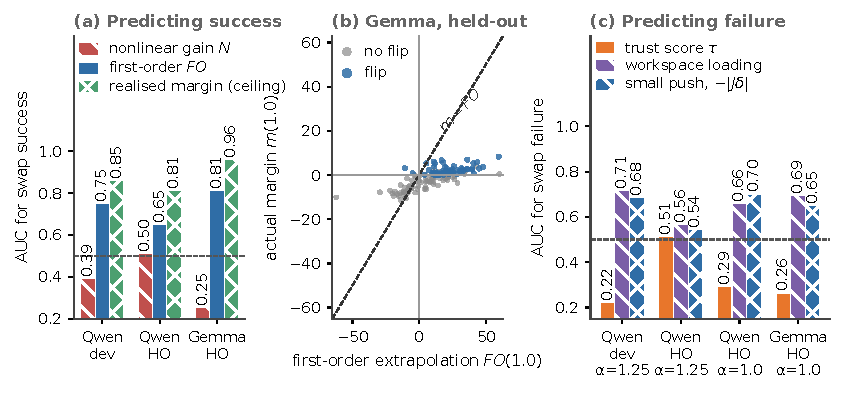
\includegraphics[width=5.63in]{figures/fig_e1.pdf}
\caption{\textbf{What predicts swap outcomes.} HO: held-out suite. (a) AUC for swap success of the nonlinear remainder $N$, the first-order extrapolation $FO$ and the realised margin (a ceiling) on three item sets. (b) Actual margin against $FO$ at the working strength on Gemma~3~12B: flips have the larger $FO$, but many non-flips also have large positive $FO$, and points lie below the diagonal (saturation). (c) AUC for swap \emph{failure}: the trust score $\tau$ (mid layer) falls below 0.5, i.e.\ high $\tau$ marks success; a small push $\|J\delta\|$ predicts failure. Qwen HO is shown at both strengths ($\alpha=1.25$ is its primary strength).}
\label{fig:e1}
\end{figure}

\textbf{The trust score tracks the size of the first-order push.} The notes behind this program predicted that high $\tau$ marks swap failure (H1). It does not. $\tau$ is a faithful linearization-error score ($\rho=0.95$ with the true first-order error), but its AUC for failure is 0.22 on the dev suite, 0.29 on Qwen held-out items at $\alpha=1.0$ and 0.26 on Gemma held-out items; values below 0.5 mean that high $\tau$ marks success (stratified $p=0.012$ on Qwen held-out at $\alpha=1.0$ and $0.007$ on Gemma for the reversal). The sign is explained by the push size: a small push $-\|J\delta\|$ predicts failure (AUC 0.70 and 0.65), and $\tau$ correlates positively with $\|J\delta\|$ (0.59 and 0.44), so large pushes have both a larger $\tau$ and more successes. At Qwen's primary strength $\alpha=1.25$ the association vanishes (AUC 0.51, \figref{fig:e1}c), consistent with $\tau$ being mostly an effect-size proxy.

\subsection{Mutual inhibition at ignition holds on one 4B model only}
\label{sec:claima}
At the point where an interpolated embedding flips the model's answer between two countries, we asked whether the two concepts inhibit each other at second order (the original work finds some competition but not whether it is sharp). On Qwen3.5-4B the answer is yes: both cross-terms are negative in 24/24 original trials and in 88\% of 120 held-out trials; inhibition at the threshold exceeds zero, exceeds its value at $\alpha^*\pm0.2$ and exceeds a random orthogonal pair (all three tests pass, $p<2\times10^{-7}$ on the original set and $<10^{-8}$ on the held-out set), while the first-order cross-effect is positive ($+0.27$ to $+0.33$), so the J-lens cannot see it. The effect does not transfer (\figref{fig:claima}a): on Gemma~3~12B only 29--30\% of trials have both terms negative and inhibition does not peak at the threshold; on Qwen3.6-27B (the same family, mixed precision) 8--17\% do and all three tests fail. An exploratory scan of 18 layer-pair and direction-source configurations per model (\figref{fig:claima}c,d) finds the effect on Qwen3.5-4B in 14 of 18 configurations with Bonferroni correction (it needs a target layer well below the output, and works with identity directions, so not only with the J-lens) and in none on Gemma (\figref{fig:claima}c,d; the identity-direction configurations are in the right-hand heatmaps). Repeating the nine J-lens configurations on the 120 held-out trials, with the prediction registered in advance, gives the same split: the six with a target layer well below the output pass all three tests (both cross-terms negative in 89--100\% of trials) and the three near the output fail the peak-at-threshold test ($p=0.2$--$0.4$, 27--37\% both-negative). The ignition threshold is selected from the same trials, which could by itself make cross-terms negative; the identical procedure finds no effect on Gemma or on the 27B, and the peak is at the threshold and not at $\alpha^*\pm0.2$, but we did not test a toy saturating-competition model, which remains open. We therefore state claim A as a finding on Qwen3.5-4B, not about lenses, a model family or language models in general.

\begin{figure}[!t]
\centering
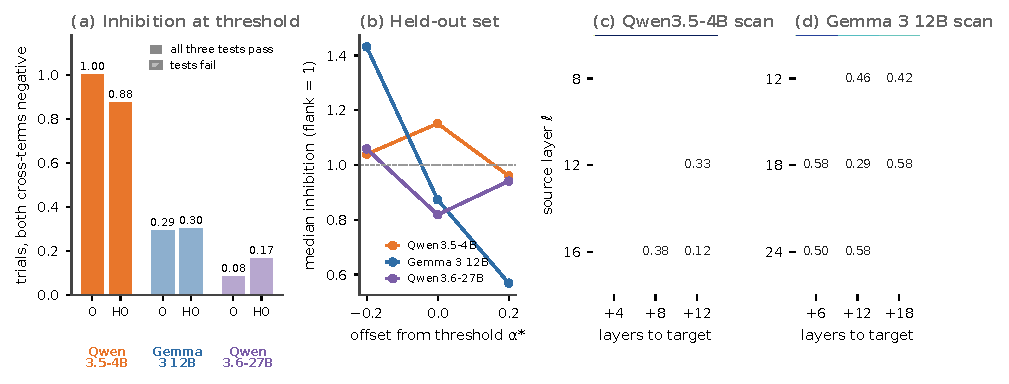
\includegraphics[width=5.91in]{figures/fig_claim_a.pdf}
\caption{\textbf{Second-order inhibition at the ignition threshold is specific to Qwen3.5-4B.} (a) Fraction of trials with both cross-terms negative at the threshold on the original (O, 24 trials) and held-out (HO, 120) sets; hatched bars: the pre-registered tests fail. (b) Median inhibition at the threshold and $\pm0.2$ on the held-out set, normalized by the flank mean; only Qwen3.5-4B peaks at the threshold. (c,d) Exploratory scan on 24 trials of source layer $\times$ layers-to-target configurations, with J-lens directions (left heatmap of each pair) and identity directions (right): fraction of trials with both cross-terms negative; $*$ marks configurations that pass all three tests with Bonferroni correction (14 of 18 on Qwen3.5-4B, 0 of 18 on Gemma).}
\label{fig:claima}
\end{figure}

\subsection{What curvature does not explain}
\label{sec:negatives}
\textbf{No motor-regime collapse.} If the late rise in lens dimensionality means $\jl\to I$, curvature in that band should collapse (H8). $\jl\to I$ holds on Qwen (distance to a scaled identity 0.996 at L0 to 0.46 at L30) and weakly on Gemma (1.00 to 0.83), but per-block nonlinearity \emph{rises} toward the output on both (motor/workspace ratio 3.73 and 5.05, intervals $[3.5,4.0]$ and $[4.7,5.6]$; the randomized models also rise, 2.06 and 2.33; \figref{fig:structure}a,b).

\begin{figure}[!t]
\centering
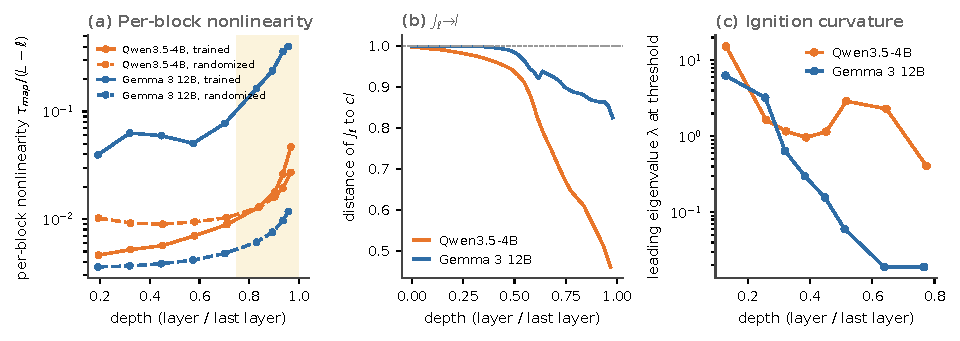
\includegraphics[width=5.97in]{figures/fig_structure.pdf}
\caption{\textbf{Nonlinearity rises toward the output; ignition curvature is not a general feature.} (a) Per-block nonlinearity of the layer-to-output map (random 10\% perturbations; trained: solid, weight-randomized: dashed). (b) Distance of the lens matrix $\jl$ to its best scalar multiple of the identity. (c) Leading Hessian eigenvalue of the commitment map at the ignition threshold, per layer (median over 24 trials with 95\% bootstrap interval). Dashed lines in (a): weight-randomized models (``random''); in (b), Gemma is dashed for legibility.}
\label{fig:structure}
\end{figure}

\textbf{Ignition as a curvature event is weak on Qwen and absent on Gemma (H6).} On Qwen the three pre-registered tests pass, but support rests on three layers (L4, L20, L24; L4 carries 78\% of the pooled statistic), layers L10--L16 show none, and at the threshold the Taylor radius has already collapsed at L16--L24 (0\% of cells valid). A Lanczos check over 320 cells shows the eigenvalues are converged (median relative error 0.01\%, decision statistic stable in 100\%), and scaling by the residual norm shrinks the L4 lead from $5.4\times$ to $1.6\times$. On Gemma the leading eigenvalue falls monotonically with depth and the tests fail (flank difference $p=0.90$; \figref{fig:structure}c).

\textbf{Binding, the remainder, early layers and load.} Hessian cross-terms of binding pairs are not special (H3: rank-fraction 0.496, $p=0.55$, 35 items; the Taylor-2 prediction of measured ablation interactions is within 50\% for 93\% of pairs). Selected sparse atoms couple slightly \emph{less} to the non-J-space remainder's curvature than best-correlated unselected atoms (H5, two forms), and a post-hoc ``orthogonality bias'' account we proposed was refuted by its own follow-up. Where the first-order lens is blind (L4), second-order curvature carries no significant content (H7: $T=0.55$, $p=0.19$; the first-order lens already reads content at L8). Inhibition among listed words does not rise with list length (H9-load; Spearman $-0.51$, i.e.\ it falls; the occupancy measure is post hoc and under-powered, so we draw no conclusion beyond ``no support'').

\textbf{A persona effect did not survive scaling.} Applying the ignition protocol to persona and register word pairs (H10), a 4-pair run suggested that persona pairs show the signature and register pairs do not, a 10-pair run replicated this, and a distance-matched object-noun control showed that unrelated objects do too. At 100 pairs per family (persona, near-synonym, matched control; plus all 66 country pairs; 732 trials; pair-level tests), all four families show a positive effect at the pair level (median $\bar D$ with 95\% bootstrap interval: persona 0.30 [0.22, 0.35], control 0.36 [0.29, 0.42], countries 0.49 [0.42, 0.62], near-synonym 0.06 [0.02, 0.11]; one-sided Wilcoxon $p<10^{-5}$ in each family; 93\%, 94\%, 97\% and 68\% of pairs positive), but near-synonyms only weakly (\figref{fig:h10}). The pre-registered primary contrast (T1: matched persona minus control, Wilcoxon over 100 pairs, threshold $p<0.01$) shows no persona excess (median pair difference $-0.043$, $p=0.08$). The secondary regression (T2) gives a persona coefficient of $-0.09$ (95\% CI $[-0.18,-0.006]$): after adjusting for endpoint distance, persona is if anything slightly lower than the control. Endpoint distance explains variation within families (Spearman $\approx0.3$) but not between them (overall 0.19); pair-level slot surprisal (how well the nouns fit the carrier), embedding similarity and word length are associated with the effect, jointly explaining 24\% of variance and none of the family gaps.

\begin{figure}[!t]
\centering
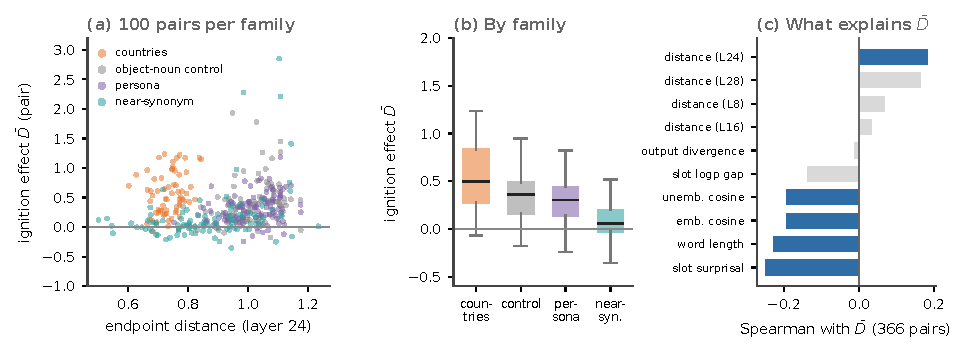
\includegraphics[width=5.79in]{figures/fig_h10.pdf}
\caption{\textbf{Persona is not special once pairs are scaled and matched.} (a) Pair-level ignition effect $\bar D$ (mean over L20 and L24 of the median over a pair's two carriers of $\lambda(\text{threshold})-\text{mean}\,\lambda(\text{flanks})$) against endpoint distance for 100 pairs per family and 66 country pairs. (b) The same by family. (c) Spearman correlation of $\bar D$ with pair-level covariates over 366 pairs (blue bars with $*$: significant after Bonferroni correction).}
\label{fig:h10}
\end{figure}

\section{Related work}
\textbf{Lens methods.} The J-lens extends the logit lens~\citep{nostalgebraist2020logit} and the tuned lens~\citep{belrose2023tuned} and is related to the mean-Jacobian relation maps of \citet{hernandez2024linearity}; a recent refinement filters Jacobians for faithfulness~\citep{ayonrinde2026jpp}, and independent work analyses the lens's readout mathematically as a short-horizon, sparse operator~\citep{yan2026short} and reads multi-token concepts from it~\citep{gong2026firsttoken}. Nanda's review of the original paper reports, in a Qwen reproduction of multi-hop recall, that swapping the answer can dominate swapping the intermediate concept, where the original work finds the opposite in workspace layers~\citep{nanda2026review}; our swaps act on the intermediate concept, and its rates vary with model and strength. We keep the lens fixed and ask what lies beyond its first-order assumption.
\textbf{Linearization and attribution.} Gradient attribution~\citep{sundararajan2017axiomatic}, attribution patching~\citep{nanda2023attribution,syed2023attribution,kramar2024atp} and attribution graphs~\citep{ameisen2025circuit,lindsey2025biology,marks2024sparse} treat the network as locally linear, an approximation that rests on the piecewise-linear structure of the network~\citep{montufar2014number,elhage2021mathematical}. Closest to ours, \citet{zhang2026lies} diagnose first-order attribution error with a second-order reliability score and an HVP correction; our trust score is the same ratio applied to concept swaps rather than patched components. Pairwise interaction attribution with Hessians~\citep{janizek2021explaining} motivates our binding tests.
\textbf{Curvature in deep learning.} HVPs~\citep{pearlmutter1994fast}, Lanczos iterations~\citep{lanczos1950iteration} and Hessian spectra of the loss~\citep{ghorbani2019investigation,yao2020pyhessian} are standard tools for the \emph{parameter} space; we apply them to \emph{activation} space, along concept directions.
\textbf{Interventions and controls.} Concept swaps, steering and activation patching~\citep{meng2022locating,turner2023activation,heimersheim2024activation} are first-order or discrete interventions; weight-randomization sanity checks~\citep{adebayo2018sanity}, equivalence tests~\citep{lakens2017equivalence} and pre-registration~\citep{nosek2018preregistration} guard the claims we make about them. The superposition and linear-representation views~\citep{elhage2022toy,park2023linear,bricken2023monosemanticity,cunningham2023sparse} frame why lens vectors are overcomplete and why a sparse decomposition over them is meaningful.

\section{Discussion}
\textbf{What we learned.} The curvature of the MLP branch is raised along J-lens directions in three architectures and absent under weight randomization, so token-aligned directions, which include the lens's, are privileged for second-order structure; variance does not explain this, but unembedding directions without the Jacobian carry nearly all of it, so the evidence does not show that the Jacobian map matters. The size of this effect varies by an order of magnitude across models (median ratio 1.3 to 9.4), which we cannot yet explain; part of Gemma's effect tracks its larger first-order gain, and a threefold gain-normalized enrichment remains. For the interventions the lens supports, the local first-order extrapolation ranks swap outcomes better than the nonlinear remainder, and the trust score marks effect size, not failure. This is not a statement that swaps are linear: success is threshold-like, and the extrapolation flags many swaps that fail. For the second-order program it localizes the contribution: curvature adds a description of the structure around lens directions, not a better predictor of what interventions do.

\textbf{Limitations.}
\begin{itemize}
\item \emph{Few models and small, templated stimuli.} Three architectures for curvature, two for swaps; claim A holds on one 4B model only (the 27B used mixed precision, validated for that one measurement on a shorter slice). The held-out suite is templated and city-dominated, and items and pairs that share words or relations are not independent, so the reported $p$-values and Wilson intervals are optimistic.
\item \emph{Post-hoc elements,} all dated: the stratified analysis, the H5 follow-up, H9-load, the Gemma working strength (confirmed out of sample), B$'$ itself (designed after B failed), and the control populations of \secref{sec:bprime} (designed after B$'$). The pre-registrations are internal: written by the same team, hash-recorded, and not deposited with a third party.
\item \emph{Measurement scope.} $\kappa$ is MLP-branch curvature at one layer at a time; lens vectors of active tokens are not independent of the residual's content, so part of the effect may be alignment with high-variance directions. Nulls use one lens-fitting recipe (30 prompts) and up to five seeds, and the real lenses were fitted on 417--1000 prompts, which differs by model; \secref{sec:bprime} tests the recipe difference directly. The ignition threshold is selected from the data that the inhibition tests use, and we did not test a saturating-competition model.
\item \emph{No causal test of use.} Nothing here shows the model uses curvature along lens directions. The conclusion that second-order measures add no rank information about swaps rests on the failure of the hypotheses we tested, on two models and templated items.
\end{itemize}

\textbf{Open questions.} A causal test of whether curvature along lens directions matters for behavior (perturbing along high-curvature directions against matched controls) is the experiment this study most needs. Why the effect is 10$\times$ larger on Gemma, why the inhibition effect is specific to one model, and what makes country pairs the strongest ignition pairs are open. Two hypotheses (automatization under reinforcement learning and reflection training) need training checkpoints we do not have.

\textbf{Reproducibility.} The code, tests, pre-registrations (with hashes), results and a step-by-step log of every bug found (a tokenizer scoring bug, per-block kwargs, Gemma's embedding scale and extra norm, a stimulus-spacing artifact, memory failures) are in the accompanying repository; Appendix~\ref{app:prereg} lists the registrations.

\bibliographystyle{plainnat}
\bibliography{refs}

\appendix
\section{Pre-registrations and result files}
\label{app:prereg}
\small
Each experiment has a pre-registration in \texttt{hlens/docs/preregistration\_*.md}, hashed into its result file: H3, H5, H6, E1, H7, H8, H9 and H10 (first runs); the replication of the gates and of H2/H9 on Gemma and Qwen (with an addendum on stimulus spacing); B$'$ and its Llama repeat; mixed-precision validation; the 27B inhibition test; H6/H8 on Gemma; the held-out swap suite; case-insensitive rescoring with H1/E1 on held-out items; E1 and H1 on Gemma; the extended, control and 100-pair H10 runs; the claim-A scan and H10 covariate study (exploratory); the Lanczos convergence check; and the control populations and extra Gemma null seeds added after review. A manifest of the SHA-256 of every registration file is in \texttt{paper/prereg\_hashes.txt} in the repository. Raw results are in \texttt{results/}; the narrative record, including every bug, is in \texttt{hlens/docs/handoff.md}.

\section{Control populations for the curvature ratio}
\label{app:controls}
Registered in \texttt{preregistration\_b\_prime\_controls.md} after B$'$ had been run. For each lens direction at layer $\ell$ we compare against: \emph{varmatch}, the activation-covariance or isotropic direction (pool of 2048) with the closest variance of the residual along it (median $|\log$ variance ratio$|$ 0.01--0.23, i.e.\ matched within 1--26\%); \emph{embed}, input-embedding rows of the same active tokens; \emph{unembed}, the unembedding gradient directions of the same tokens (the lens vectors without $J_\ell$); and \emph{cov}, directions sampled from the second-moment matrix of 1,200 residual activations from disjoint prompts. All use the B$'$ evaluation prompts, 16 contexts per prompt, 64 directions and the prompt-cluster bootstrap; the lens and random populations reproduce the stored B$'$ ratios. A test passes when the lower bound of the lens-to-control ratio exceeds 1.05 at at least 75\% of layers at depth $\ge0.5$.
\begin{table}[h]
\centering\small
\begin{tabular}{@{}lllll@{}}
\toprule
Model & varmatch & embed & unembed & cov (descriptive) \\
\midrule
Qwen3.5-4B & 1.32 (8/8) & 1.17 (8/8) & 1.16 (8/8) & 1.01 (2/8) \\
Gemma 3 12B & 9.23 (6/6) & 6.67 (6/6) & 1.05 (3/6) & 129 (6/6) \\
Llama 3.1 8B & 1.40 (8/8) & 1.40 (8/8) & 1.32 (8/8) & 1.26 (8/8) \\
\bottomrule
\end{tabular}
\caption{\label{tab:controls}Median over layers (depth $\ge0.5$) of the ratio $\kappa(\text{lens})/\kappa(\text{control})$, with the number of layers whose interval lower bound exceeds 1.05. Variance matching (V) passes on all three models. The token-direction test (K) passes for embed and unembed on Qwen and Llama and fails for unembed on Gemma (ratio 1.05). The cov control has 129$\times$ lower curvature than the lens on Gemma, so its ratio is large; on Qwen it is about 1.}
\end{table}

\section{Held-out swap suite}
\label{app:swap}
Figure~\ref{fig:swap} gives the swap rates and the per-relation breakdown on the 165-item held-out suite (\secref{sec:suffice}).
\begin{figure}[h]
\centering
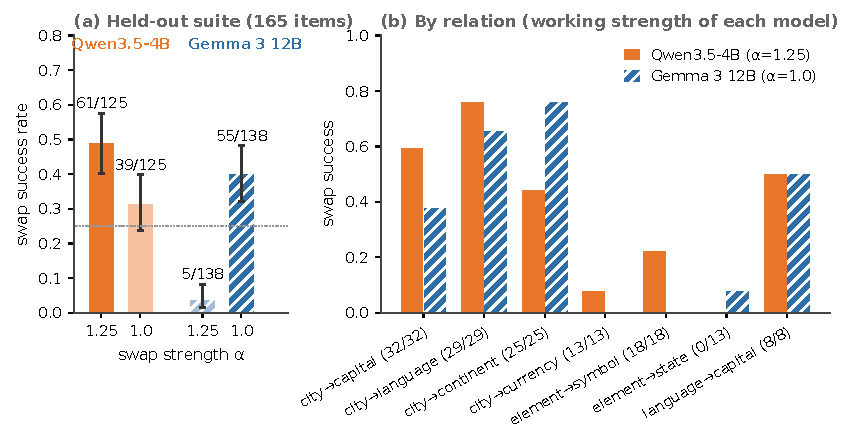
\includegraphics[width=5.69in]{figures/fig_swap.pdf}
\caption{\textbf{Concept swaps on a held-out suite.} (a) Fraction of baseline-correct items whose answer flips to the swapped answer, with Wilson 95\% intervals and counts; random-direction controls flip 0 items in all four settings (gray bars, not visible). The faint bars are the non-working strengths; the dotted line is the pre-registered pass threshold (25\%). (b) The same by relation at each model's working strength; labels give the number of items (Qwen/Gemma).}
\label{fig:swap}
\end{figure}

\section{Effect sizes with intervals}
\label{app:effects}
\begin{table}[h]
\centering\footnotesize
\begin{tabular}{@{}p{2.9cm}p{5.1cm}p{1.9cm}p{2.2cm}p{2.3cm}@{}}
\toprule
Model & Quantity & Estimate & 95\% interval & Interval method \\
\midrule
Qwen3.5-4B & B$'$: $\kappa$ ratio at L30 & 2.20 & [2.15, 2.24] & prompt-cluster bootstrap \\
Gemma 3 12B & B$'$: $\kappa$ ratio at L44 & 12.99 & [12.58, 13.45] & prompt-cluster bootstrap \\
Llama 3.1 8B & B$'$: $\kappa$ ratio at L30 & 2.83 & [2.75, 2.92] & prompt-cluster bootstrap \\
Qwen3.5-4B & swap success, $\alpha=1.25$ (held-out) & 0.49 (61/125) & [0.40, 0.57] & Wilson, items \\
Gemma 3 12B & swap success, $\alpha=1.0$ (held-out) & 0.40 (55/138) & [0.32, 0.48] & Wilson, items \\
Qwen3.5-4B (dev) & AUC of $N$ (success) & 0.39 & [0.23, 0.56] & bootstrap, items \\
Qwen3.5-4B (dev) & AUC of $FO$ (success) & 0.75 & [0.60, 0.87] & bootstrap, items \\
Qwen3.5-4B (HO) & AUC of $N$ (success) & 0.50 & [0.40, 0.60] & bootstrap, items \\
Qwen3.5-4B (HO) & AUC of $FO$ (success) & 0.65 & [0.54, 0.74] & bootstrap, items \\
Gemma 3 12B (HO) & AUC of $N$ (success) & 0.25 & [0.17, 0.33] & bootstrap, items \\
Gemma 3 12B (HO) & AUC of $FO$ (success) & 0.81 & [0.73, 0.88] & bootstrap, items \\
Qwen3.5-4B (dev) & AUC of $\tau$ (failure) & 0.22 & [0.10, 0.35] & bootstrap, items \\
Qwen3.5-4B (HO, $\alpha=1.0$) & AUC of $\tau$ (failure) & 0.29 & [0.20, 0.39] & bootstrap, items \\
Qwen3.5-4B (HO, $\alpha=1.25$) & AUC of $\tau$ (failure) & 0.51 & [0.40, 0.61] & bootstrap, items \\
Gemma 3 12B (HO) & AUC of $\tau$ (failure) & 0.26 & [0.18, 0.34] & bootstrap, items \\
Qwen3.5-4B & both cross-terms negative (O, n=24) & 1.00 & [0.86, 1.00] & Wilson, trials \\
Qwen3.5-4B & both cross-terms negative (HO, n=120) & 0.88 & [0.80, 0.92] & Wilson, trials \\
Gemma 3 12B & both cross-terms negative (O, n=24) & 0.29 & [0.15, 0.49] & Wilson, trials \\
Gemma 3 12B & both cross-terms negative (HO, n=120) & 0.30 & [0.23, 0.39] & Wilson, trials \\
Qwen3.6-27B & both cross-terms negative (O, n=24) & 0.08 & [0.02, 0.26] & Wilson, trials \\
Qwen3.6-27B & both cross-terms negative (HO, n=120) & 0.17 & [0.11, 0.24] & Wilson, trials \\
Qwen3.5-4B & H10 median $\bar D$, persona (100 pairs) & 0.30 & [0.23, 0.35] & bootstrap, pairs \\
Qwen3.5-4B & H10 median $\bar D$, object-noun control (100 pairs) & 0.36 & [0.29, 0.42] & bootstrap, pairs \\
Qwen3.5-4B & H10 median $\bar D$, countries (66 pairs) & 0.49 & [0.42, 0.62] & bootstrap, pairs \\
Qwen3.5-4B & H10 median $\bar D$, near-synonym (100 pairs) & 0.06 & [0.02, 0.11] & bootstrap, pairs \\
\bottomrule
\end{tabular}
\caption{Effect sizes behind the headline results. HO: held-out. AUC intervals are item bootstraps (2,000 resamples) and do not account for items sharing relations or entities, so they are optimistic. The $\kappa$ ratio rows give the last measured layer.}
\end{table}

\section{Reproduction of first-order checks}
\label{app:gates}
\begin{table}[h]
\centering\small
\begin{tabular}{@{}p{4.3cm}p{5.4cm}p{5.2cm}@{}}
\toprule
Check & Qwen3.5-4B & Gemma 3 12B \\
\midrule
Workspace range (landmarks) & depth $\approx0.3$--$0.9$ & depth 0.43--0.91 (L20--43) \\
Sparse decomposition (J-space variance) & 7--9\% at L12/16/20 (random atoms: 15\%) & --- \\
Context-free MLP gain & not reproduced (8.3$\times$ at L30 only) & --- \\
Swap, original suite (87/89 items) & 35\% (random 0/52) & 17\% at $\alpha=1.25$; 29\% at $\alpha=1.0$ (post hoc); original suite, not the held-out suite of \secref{sec:suffice} (3.6\% and 39.9\%) \\
Early averaging (restricted Hessians) & ratio 0.35 vs null 0.11; randomized 0.29 & --- \\
\bottomrule
\end{tabular}
\caption{First-order checks and the early-averaging test (is an \emph{averaged} Hessian object meaningful?). A randomized network gives a similar ratio, so we make no claim about an averaged H-lens.}
\end{table}

\section{The failed first formulation of the curvature test (B)}
\label{app:b}
Pre-registered rules: T1 (lens/random ratio CI above 1 in $\ge75\%$ of layers at depth $\ge0.5$), T2 (median ratio $\ge1.5$) and T3 (null interval contains 1). T1 held on both models; T2 failed on Qwen (1.37); T3 failed in 7 of 8 null arms because intervals about $\pm0.0005$ wide excluded 1 at ratios 0.997--1.002. B$'$ replaced T3 by the equivalence margin and dropped T2 from the pass rule (the median is reported and ``large'' requires 1.5).

\section{Mixed precision and Lanczos checks}
A bf16 model with fp32 slice, final norm and head reproduced the full-fp32 inhibition result on Qwen3.5-4B over 24 trials $\times$ 3 offsets (all pre-registered criteria: sign agreement 98.6\%/100\%, Spearman 0.9987, median relative error 0.34\%, 90th percentile 0.96\%, identical test outcomes, thresholds within 0.05 in 24/24). Eight-iteration Lanczos eigenvalues agreed with 40-iteration references to a median 0.01\% (90th percentile 0.7\%, maximum 17.8\%); the 16-iteration estimate equals the 40-iteration one to numerical precision.

\section{Pitfalls we hit}
Counting the bare-space token made numeric answers overlap and swap margins identically zero (fixed; all swap results re-run, headline AUCs moved $\le0.03$). Reusing one block's rotary and mask kwargs for a whole slice gave errors of 4--5.5. Capturing slice kwargs inside a function transform crashed on reuse. Gemma multiplies embeddings by $\sqrt d$ and has a post-feedforward norm. A double space before the slot is split by one tokenizer and merged by another. A null rule of ``interval contains 1'' fails when intervals are narrow. A 10-pair persona/register contrast vanished at 100 pairs. Unsaved long runs were lost to memory events and reboots, motivating per-trial checkpointing.

\end{document}
